% !TEX program = xelatex
%% Requires compilation with XeLaTeX or LuaLaTeX
\documentclass[10pt,xcolor={table,dvipsnames},t]{beamer}
\usepackage{biblatex}
\usepackage{caption}
\setbeamertemplate{caption}[numbered]
\addbibresource{reference.bib}
\usepackage{hyperref}
\hypersetup{ 
pdfpagemode=FullScreen,  
colorlinks=true,linkcolor=blue}
\usepackage{enumerate}
\usepackage{algorithm}
\usepackage{algpseudocode}
\usepackage{listings}
\usepackage{xcolor}

\definecolor{codegreen}{rgb}{0,0.6,0}
\definecolor{codegray}{rgb}{0.5,0.5,0.5}
\definecolor{codepurple}{rgb}{0.58,0,0.82}
\definecolor{backcolour}{rgb}{0.95,0.95,0.92}

\lstdefinestyle{mystyle}{
    backgroundcolor=\color{backcolour},   
    commentstyle=\color{codegreen},
    keywordstyle=\color{magenta},
    numberstyle=\tiny\color{codegray},
    stringstyle=\color{codepurple},
    basicstyle=\ttfamily\footnotesize,
    breakatwhitespace=false,         
    breaklines=true,                 
    captionpos=b,                    
    keepspaces=true,                 
    numbers=left,                    
    numbersep=5pt,                  
    showspaces=false,                
    showstringspaces=false,
    showtabs=false,                  
    tabsize=2
}

\lstset{style=mystyle}

% Flow chart config
\usepackage{tikz}
\usetikzlibrary{calc,trees,positioning,arrows,fit,shapes,calc,tikzmark,matrix}
\usepackage{eso-pic}
\usetikzlibrary{shapes.geometric, arrows}
\tikzstyle{startstop} = [rectangle, rounded corners, minimum width=3cm, minimum height=1cm,text centered, draw=black, fill=red!30]
\tikzstyle{io} = [trapezium, trapezium left angle=70, trapezium right angle=110, minimum width=3cm, minimum height=1cm, text centered, draw=black, fill=blue!30]
\tikzstyle{process} = [rectangle, minimum width=3cm, minimum height=1cm, text centered, draw=black, fill=orange!30]
\tikzstyle{decision} = [diamond, minimum width=3cm, minimum height=1cm, text centered, draw=black, fill=green!30]
\tikzstyle{arrow} = [thick,->,>=stealth]

\usetheme{UCBerkeley}

\title[Your Short Title]{STMC HKOI Training}
\subtitle{Lesson 6: Looping structure and arrays (II)}
\author{Chan Yan Mong}
%\institute{}
\date{\today}

\begin{document}

\begin{frame}
  \titlepage
\end{frame}

% Uncomment these lines for an automatically generated outline.
%\begin{frame}{Outline}
%  \tableofcontents
%\end{frame}

\section{Class Goal}

\begin{frame}{Goal today}
Today we will look at more list features and see how we can combine it with loops to do more advance applications
\begin{itemize}
  \item List slicing, concatenation and membership
  \item Multiple dimensions list
  \item Loop breaks
  \item Many applications:
  \begin{itemize}
    \item Bomberman Solver 
    \item Fisher-Yates shuffle algorithm
    \item Linear Search
    \item Maximum Subarray Sum
  \end{itemize}
\end{itemize}

\end{frame}


\section{List operations}
\subsection{List Membership}
\begin{frame}[fragile]{List: Membership}
  \begin{itemize}
    \item Sometimes we want to check if a member belongs to a list
    \item Python provide us with an easy way to do it using \texttt{in} keyword
    \item Here are some examples:
\begin{lstlisting}[language=python]
  >> 3 in [1,2,3]
  True
  >> "Tim" in ['John','Jerry','May']
  False
\end{lstlisting}
  \end{itemize}
\end{frame}

\subsection{List Concatenation}
\begin{frame}[fragile]{List: Concatenation}
  \begin{itemize}
    \item We can also \textit{"add"} two list by joining them together
    \item This is called \textbf{concatenation}
    \item This is done using the \texttt{+} operator
    \item For example:
\begin{lstlisting}[language=python]
  >> [4,5,6] + [1,2,3]
  [4,5,6,1,2,3]
  >> ["Tim","Katy"] + ['John','Jerry','May']
  ['Tim', 'Katy', 'John', 'Jerry', 'May']
\end{lstlisting}
  \end{itemize}
\end{frame}

\subsection{List Slicing}
\begin{frame}[fragile]{List: Slicing}
  \begin{itemize}
    \item Sometimes we want to make a copy of \textit{part} of the list
    \item This operation is called \textbf{slicing}
    \item The basic syntax of slicing is:
\begin{lstlisting}[language=python]
  mylist[start:end]
\end{lstlisting}
    \item The slice \textbf{includes start but exclude end}
  \end{itemize}
\end{frame}

\begin{frame}[fragile]{List: Slicing}
  \begin{itemize}
    \item Here are some examples:
    \begin{lstlisting}[language=python]
mylist = [0,1,2,3,4,5,6]

mylist[0:1] # Return [0]
mylist[0:3] # Return [0,1,2]
mylist[3:5] # Return [3,4]
mylist[1:5] # Return [1,2,3,4]
\end{lstlisting}
  \end{itemize}
\end{frame}

\begin{frame}[fragile]{List: Slicing}
  \begin{itemize}
    \item One can also either start or end as blank
    \item If start is left blank, it's equivalent as putting zero as start 
    \item If end is left blank, it's equivalent as putting \texttt{len(<the list you slice>)} as end
    \item More explicitly
\begin{lstlisting}[language=python]
  mylist[:4] # Same as mylist[0:4]
  mylist[3:] # Same as mylist[3:len(mylist)]
\end{lstlisting}
  \end{itemize}
  
\end{frame}

\begin{frame}[fragile]{List: Slicing}
  \begin{itemize}
    \item Here are some explicit examples:
\begin{lstlisting}[language=python]

  mylist = [0,1,2,3,4,5,6]
  
  mylist[:4] # Same as mylist[0:4] so [0, 1, 2, 3]
  mylist[2:] # Same as mylist[2:len(mylist)] so [2, 3, 4, 5, 6]
  \end{lstlisting}
  \end{itemize}
\end{frame}

\begin{frame}[fragile]{List: Slicing}
  \begin{itemize}
    \item We can also specify the interval of slicing via the following syntax:
\begin{lstlisting}[language=python]
  mylist[0:6:2] # This will give [0,2,4]
  mylist[1:6:2] # This will give [1,3,5]
  mylist[2:6:2] # This will give [2,4]
  mylist[2:6:3] # This will give [2,5]
\end{lstlisting}
  \item Again, you can see the end is always excluded
  \end{itemize}
\end{frame}

\subsection{Multidimensional List}
\begin{frame}[fragile]{List: Multidimensional List}
  \begin{itemize}
    \item We can also put list inside list to create multidimensional lists (Or multidimensional array as other language will call)
    \item For example, the following is a 2-dimensional array with $3$ rows and $4$ columns. We shall denote such array \texttt{List(3,4)}
    \begin{align*}
      \left[
      \begin{array}{cccc}
        \rowcolor{red!0}
        1 & 2 & 3 & 4 \\
        \rowcolor{red!0}
        5 & 6 & 7 & 8\\
        \rowcolor{red!0}
        9 & 10 & 11 & 12\\
      \end{array}
      \right]
    \end{align*}
  \end{itemize}
\end{frame}

\begin{frame}[fragile]{List: Multidimensional List}
  \begin{itemize}
    \item One can implement the list above using the following python code:
  \end{itemize}
\begin{lstlisting}[language=python]
twoDim = [
  [1,2,3,4],
  [5,6,7,8],
  [9,10,11,12]
]

# Be careful about the order of the index 
twoDim[0]    # [1,2,3,4]
twoDim[1]    # [5,6,7,8]
twoDim[0][0] # 1
twoDim[1][0] # 5
twoDim[0][2] # 3
twoDim[2][3] # 12
\end{lstlisting}
\end{frame}


\begin{frame}[fragile]{List: Multidimensional List}
  \begin{itemize}
    \item We can also go higher dimension by keep wrapping list inside list. For example to create a list of form \texttt{List(2,2,2)}
  \end{itemize}
\begin{lstlisting}[language=python]
threeDim = [
  [
    [0,1],
    [2,3]
  ],
  [
    [4,5],
    [6,7]
  ]
]
\end{lstlisting}
\end{frame}

\section{Bomberman Solver}
\begin{frame}{Example: Bomberman (I)}
  \textbf{Reference: Ch.3 Sec.2 \textit{"Aha! Visualizing Algorithms: The Basics"} (ISBN: 9863474363)}
  \begin{columns}
    \column{0.6\textwidth}
    \begin{itemize}
      \item Bomberman is an arcade-style maze-based video game developed by Hudson Soft on 1983.
      \item Since then multiple versions of the game have been released and it remained on the classics
      \item In the game, players have to place bombs in certain locations to remove walls and eliminate all enemies from the map
    \end{itemize}
    \column{0.4\textwidth}
    \begin{figure}
      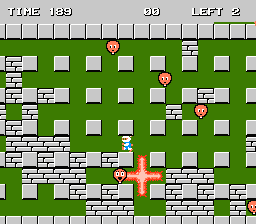
\includegraphics[width=\textwidth]{img/bomberman_nes.png}
    \end{figure}
  \end{columns}
\end{frame}

\begin{frame}{Example: Bomberman (I)}
  \begin{itemize}
    \item We will now consider a simplified version of the game to explore what we can do with list
    \item We will make the following simplifications:
    \begin{enumerate}
      \item The player only has one bomb
      \item The bomb is incredibly powerful. It blows up everything along the row and column it's placed and only stop when it hits a wall 
      \item All walls are unbreakable
      \item Enemies will not move
    \end{enumerate}
    \item Now we ask a question: \textbf{\textit{Given a map of walls and enemies, where can I put the bomb such that the largest number of enemies are eliminated?}}
  \end{itemize}
\end{frame}

\begin{frame}{Example: Bomberman (I)}
  
  \begin{columns}
    \column{0.6\textwidth}
    We will now formulate the problem:
    \begin{itemize}
      \item \texttt{map[n][m]} is a $n\times m$ grid index from 0
      \item Each grid holds a number from $0-2$:
      \begin{itemize}
        \item $0$ are empty showspaces 
        \item $1$ are walls 
        \item $2$ are enemies
      \end{itemize}
      \item A bomb can only be placed on grid that holds $0$
      \item For simplicity we will always make the outmost part of the list walls
    \end{itemize}
    \column{0.4\textwidth}
    For example, a $6\times 8$ play grid can look like:
    \begin{align*}
      \left[
      \begin{array}{cccccccc}
        \rowcolor{red!0}
        1 & 1 & 1 & 1 & 1 & 1 & 1 & 1 \\
        \rowcolor{red!0}
        1 & 0 & 2 & 0 & 1 & 0 & 0 & 1 \\
        \rowcolor{red!0}
        1 & 1 & 1 & 0 & 1 & 2 & 0& 1 \\
        \rowcolor{red!0}
        1 & 0 & 2 & 0 & 2 & 0 & 1 & 1 \\
        \rowcolor{red!0}
        1 & 0 & 0 & 1 & 1 & 0 & 0 & 1 \\
        \rowcolor{red!0}
        1 & 1 & 1 & 1 & 1 & 1 & 1 & 1 
      \end{array}
      \right]
    \end{align*}
  \end{columns}
\end{frame}

\begin{frame}{Example: Bomberman (I)}
  What happens if we place a bomb? For example, let's say we placed a bomb in \texttt{map[3][1]}
  \begin{align*}
    \left[
    \begin{array}{cccccccc}
      \rowcolor{red!0}
      1 & 1 & 1 & 1 & 1 & 1 & 1 & 1 \\
      \rowcolor{red!0}
      1 & 0 & 2 & 0 & 1 & 0 & 0 & 1 \\
      \rowcolor{red!0}
      1 & 1 & 1 & 0 & 1 & 2 & 0& 1 \\
      \rowcolor{red!0}
      1 & \fcolorbox{black!0}{green!30}{$0$} & 2 & 0 & 2 & 0 & 1 & 1 \\
      \rowcolor{red!0}
      1 & 0 & 0 & 1 & 1 & 0 & 0 & 1 \\
      \rowcolor{red!0}
      1 & 1 & 1 & 1 & 1 & 1 & 1 & 1 
    \end{array}
    \right]
  \end{align*}
\end{frame}


\begin{frame}{Example: Bomberman (I)}
  Then it will destroy everything in the red block
  \begin{align*}
    \left[
    \begin{array}{cccccccc}
      \rowcolor{red!0}
      1 & 1 & 1 & 1 & 1 & 1 & 1 & 1 \\
      \rowcolor{red!0}
      1 & 0 & 2 & 0 & 1 & 0 & 0 & 1 \\
      \rowcolor{red!0}
      1 & 1 & 1 & 0 & 1 & 2 & 0& 1 \\
      \rowcolor{red!0}
      1 & \fcolorbox{black!0}{green!30}{$0$} & \fcolorbox{black!0}{red!30}{$2$} & \fcolorbox{black!0}{red!30}{$0$} & \fcolorbox{black!0}{red!30}{$2$} & \fcolorbox{black!0}{red!30}{$0$} & 1 & 1 \\
      \rowcolor{red!0}
      1 & \fcolorbox{black!0}{red!30}{$0$} & 0 & 1 & 1 & 0 & 0 & 1 \\
      \rowcolor{red!0}
      1 & 1 & 1 & 1 & 1 & 1 & 1 & 1 
    \end{array}
    \right]
  \end{align*}
\end{frame}

\begin{frame}{Example: Bomberman (I)}
  Now we can restate our problem
  \begin{exampleblock}{Bomberman (I)}
    Let \texttt{grid[m][n]} be a $m\times n$ grid with walls and enemies defined above. If we can only put one bomb on an empty grid, what is the best position such that we can eliminate most enemies?
  \end{exampleblock}
  To solve that, we will use \textit{brute-force searching}
\end{frame}

\begin{frame}{Example: Bomberman (I)}
  \begin{itemize}
    \item \textbf{Brute-force searching} is a algorithmic paradigm that consists of systematically enumerating all possible candidates for the solution and checking whether each candidate satisfies the problem's statement. 
    \item In short, it means finding the solution by checking all possible combinations
    \item Although brute-force searching is the easiest to implement, it's also often the slowest to run 
    \item However, it is a good starting point for small problems
  \end{itemize}
\end{frame}

\begin{frame}{}
  \begin{algorithm}[H]
    \caption{Bomberman Solver}\label{alg:bomberman_solver}
    \begin{algorithmic}[1]
      \State{\textit{best\_cell} $\gets$ \textit{None}}
      \State{\textit{max\_kill} $\gets$ 0}

      \ForAll{\textit{cell} \textbf{in} \textit{grid}}
      \If {\textit{cell} \textbf{is empty}}
        \State{Place bomb at \textit{cell}}
        \State{\textit{kill\_count} $\gets$ Get kill count for cell}
        \If {\textit{kill\_count} > \textit{max\_kill}}
          \State{\textit{max\_kill} $\gets$ \textit{kill\_count}}
          \State{\textit{best\_cell} $\gets$ \textit{cell} }
        \EndIf
        \State{Remove bomb at \textit{cell}}
      \EndIf
    \EndFor
    \end{algorithmic}
  \end{algorithm}
\end{frame}

\section{Fisher-Yates shuffle}
\begin{frame}{Example: Card shuffling}
  \begin{columns}
    \column{0.6\textwidth}
    \begin{itemize}
      \item Suppose you want to write a poker game in computer
      \item One essential element of a poker game will be to shuffle the cards
      \item \textit{How can you produce a random permutation of cards efficiently?}
    \end{itemize}
    \column{0.4\textwidth}
    \begin{figure}
      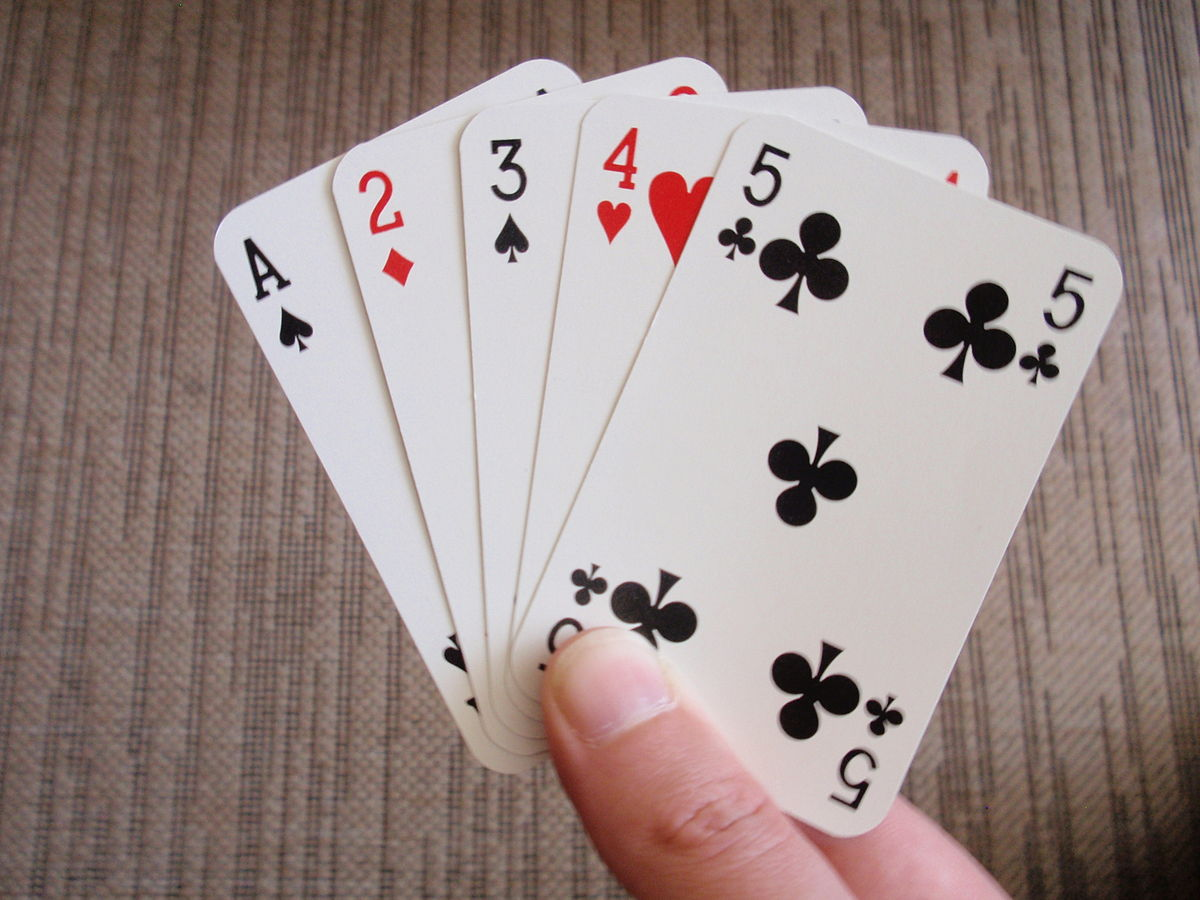
\includegraphics[width=\textwidth]{./img/poker_cards.JPG}
    \end{figure}
  \end{columns}
\end{frame}

\begin{frame}{Fisher-Yates shuffle}
  \begin{itemize}
    \item An efficient way to do it is to use the \textbf{Fisher-Yates algorithm}
    \item The idea is related to how we actually shuffle cards
    \item Suppose we have $3$ cards and we want to put them in random order 
    \item Each time we will draw one out, and place it one after another 
    \item We don't need to check if there are repetition, because the card drawn out is \textbf{removed}
    \item This insight lead to the following algorithm
  \end{itemize}
\end{frame}

\begin{frame}{Fisher-Yates shuffle}
  \begin{algorithm}[H]
    \caption{Fisher-Yates shuffle}\label{alg:fisher_yates}
    \begin{flushleft}
      \textbf{Input:} $Items$ - List of length $n$\\
      \textbf{Output:} Shuffled list of length $n$\\
      \textbf{Program:} 
    \end{flushleft}
    \begin{algorithmic}
      \ForAll {$i=0$ to $n-2$} 
        \State{$j \gets $ Random number from $i$ to $n-1$} (inclusive)
        \State{Swap $Items[i]$ and $Items[j]$}
      \EndFor
    \end{algorithmic}
  \end{algorithm}
\end{frame}

\begin{frame}{Fisher-Yates shuffle}
  \begin{itemize}
    \item Let's actually shuffle one array using the algorithm to see how it works
    \item Consider the following list of numbers:
    \begin{align*}
      \rowcolors{1}{}{}
      \begin{bmatrix}
        1 & 2 & 3 & 4
      \end{bmatrix}
    \end{align*}
    \item Now because the length of the array is 4, $n = 4$. 
    \item Also, when we first begin the loop $i=0$ so we draw a number between $0-3$
    
  \end{itemize}  
\end{frame}

\begin{frame}{Fisher-Yates shuffle}
  \begin{itemize}
    \item Let's say we draw $j=2$, then according to the algorithm we have to swap item $0$ and $2$, that is:
    \begin{gather*}
      \rowcolors{1}{}{}
      \begin{bmatrix}
        \fcolorbox{black!0}{red!30}{$1$} & 2 & \fcolorbox{black!0}{green!30}{$3$} & 4
      \end{bmatrix}\\
      \downarrow\\
      \rowcolors{1}{}{}
      \begin{bmatrix}
        \fcolorbox{black!0}{green!30}{$3$} & 2 & \fcolorbox{black!0}{red!30}{$1$} & 4
      \end{bmatrix}
    \end{gather*}
    \item This completed the first loop and $i=1$ now
  \end{itemize}
\end{frame}

\begin{frame}{Fisher-Yates shuffle}
  \begin{itemize}
    \item Now since $i=1$, according to the algorithm we should draw $j$ in between $1-3$ (Instead of $0-3$ in last run)
    \item So you can see that element 0 has been fixed. No later steps in the algorithm can change it's position. 
  \end{itemize}
  \begin{align*}
    \rowcolors{1}{}{}
      \begin{bmatrix}
        \fcolorbox{black!0}{gray!30}{$3$} & 2 & 1 & 4
      \end{bmatrix}
  \end{align*}
\end{frame}

\begin{frame}{Fisher-Yates shuffle}
  \begin{itemize}
    \item Suppose now we draw $j=3$, then according to the algorithm we have to swap $i=1$ and $j=3$, that is:
    \begin{gather*}
      \rowcolors{1}{}{}
      \begin{bmatrix}
        \fcolorbox{black!0}{gray!30}{$3$} & \fcolorbox{black!0}{red!30}{$2$} & 1 & \fcolorbox{black!0}{green!30}{$4$}
      \end{bmatrix}\\
      \downarrow\\
      \rowcolors{1}{}{}
      \begin{bmatrix}
        \fcolorbox{black!0}{gray!30}{$3$} & \fcolorbox{black!0}{green!30}{$4$} & 1 & \fcolorbox{black!0}{red!30}{$2$}
      \end{bmatrix}\\
      \downarrow\\
      \rowcolors{1}{}{}
      \begin{bmatrix}
        \fcolorbox{black!0}{gray!30}{$3$} & \fcolorbox{black!0}{gray!30}{$4$} & 1 & \fcolorbox{black!0}{red!0}{$2$}
      \end{bmatrix}
    \end{gather*}
  \end{itemize}
\end{frame}

\begin{frame}{Fisher-Yates shuffle}
  \begin{itemize}
    \item Now $i=2$ and $j$ is a random number from $2-3$. Suppose this time $j$ is $2$. Then we need to wap element $2$ with itself (i.e. not swapping)
    \begin{gather*}
      \rowcolors{1}{}{}
      \begin{bmatrix}
        \fcolorbox{black!0}{gray!30}{$3$} & \fcolorbox{black!0}{gray!30}{$4$} & \fcolorbox{black!0}{red!30}{$1$} & \fcolorbox{black!0}{red!0}{$2$}
      \end{bmatrix}\\
      \downarrow\\
      \rowcolors{1}{}{}
      \begin{bmatrix}
        \fcolorbox{black!0}{gray!30}{$3$} & \fcolorbox{black!0}{gray!30}{$4$} & \fcolorbox{black!0}{red!30}{$1$} & \fcolorbox{black!0}{red!0}{$2$}
      \end{bmatrix}\\
      \downarrow\\
      \rowcolors{1}{}{}
      \begin{bmatrix}
        \fcolorbox{black!0}{gray!30}{$3$} & \fcolorbox{black!0}{gray!30}{$4$} & \fcolorbox{black!0}{gray!30}{$1$} & \fcolorbox{black!0}{red!0}{$2$}
      \end{bmatrix}
    \end{gather*}
  \end{itemize}
\end{frame}

\begin{frame}{Fisher-Yates shuffle}
  \begin{itemize}
    \item But now $i=4-2=2$ so the algorithm said we are done! 
    \item This make sense because we only have one element left: If we have permuted element $1$ to $n-1$, then autoamtically the $n$th element will also falls in place because there is only one slot left in the queue 
    \item So finally our shuffled list is:
    \begin{gather*}
      \rowcolors{1}{}{}
      \begin{bmatrix}
        \fcolorbox{black!0}{gray!30}{$3$} & \fcolorbox{black!0}{gray!30}{$4$} & \fcolorbox{black!0}{gray!30}{$1$} & \fcolorbox{black!0}{gray!30}{$2$}
      \end{bmatrix}
    \end{gather*}
  \end{itemize}
\end{frame}


\begin{frame}[fragile]{Python implementation}
  \begin{lstlisting}[language=python]
  # Fisher-Yates shuffle in python 
  # Items - List of length n
  import random
  
  for i in range(len(Items)-1):
    j = random.randint(i,len(Items)-1) # Get random number 
    
    # Swapping 
    temp = Items[i]
    Items[i] = Items[j]
    Items[j] = temp
  \end{lstlisting}
  \end{frame}  

\begin{frame}{Correctness and Complexity}
  \begin{itemize}
    \item As one can easily see, the method does produce a randomly permuted list
    \item Furthermore to shuffle a list of $n$ we need to loop $n-1$ times 
    \item So when $n$ is large, the number of steps we need is roughly $n$ (i.e. $\mathcal{O}(n)$)
  \end{itemize}
\end{frame}

\section{Permutation and Factorials}
\begin{frame}{Permutations}
  \begin{itemize}
    \item Now the previous problem also raised an interesting question: How many \textbf{permutation} are there in general?
    \item A permutation refers to the rearrangement of orders of a set of objects
    \item Order matters (Unlike combinations)
    \item For example, the following all the different permutations of three numbers $\{A,B,C\}$
    \begin{align*}
      \{A,B,C\},\{A,C,B\}\\
      \{B,A,C\},\{B,C,A\}\\
      \{C,A,B\},\{C,B,A\}
    \end{align*}
  \end{itemize}
\end{frame}

\begin{frame}{Counting Permutations}
  \begin{itemize}
    \item In general, if we have $n$ distinct objects, what is the number of permutations?
    \item We can count this way:
    \begin{enumerate}
      \item Imagine putting the $n$ objects in queue
      \item Consider the 1st element in the queue. Since we $n$ objects, there are $n$ choice.
      \item Consider the 2nd element. We are left with $n-1$ objects, so there are $n-1$ choice. 
      \item Consider the 3rd element. We are left with $n-2$ objects, so there are $n-2$ choices 
      \item $\cdots$
    \end{enumerate}
    \item One can quickly see the total number of ways is $n\times(n-1)\times(n-2)\times\cdots 3\times 2\times 1$
  \end{itemize}
\end{frame}

\begin{frame}{Counting Permutations}
  \begin{itemize}
    \item We can also generalize this counting strategy to the case when we have $n$ distinct objects, but only $r$ slots
    \item For example, if we want to form a queue of $3$ out of $5$ students, we can count the following way:
    \begin{enumerate}
      \item For the 1st position, there are $5$ possibilities
      \item For the 2nd position, there are $4$ possibilities 
      \item For the 3rd position, there are $3$ possibilities
      \item So totally we have $5\times4\times3=36$ ways of doing it
    \end{enumerate}
    \item One can see readily see the general formula is: $n\times(n-1)\cdots\times(n-r+2)\times(n-r+1)$ 
  \end{itemize}
\end{frame}

\begin{frame}{Permutations}
  To summarize
  \begin{theorem}[Permutations of $n$ distinct objects]
    The number of ways to form a queue of length $n$ using $n$ distinct objects is:
    \begin{align*}
      n\times(n-1)\times(n-2)\cdots \times 2\times 1
    \end{align*}
    We can also write it as $n!$ to save space. This symbol pronouced as \textbf{n factorial}.
  \end{theorem}
\end{frame}

\begin{frame}{Permutations}
  \begin{theorem}[Permutations of $n$ distinct objects in $r$ slots]
    The number of ways to form a queue of length $r$ using $n$ distinct objects is:
    \begin{align*}
      P^n_r &= \frac{n!}{(n-r)!}\\ &
      = n(n-1)\cdots(n-r+2)(n-r+1)
    \end{align*}
    The symbol $P^n_r$ is called the \textbf{r-permutation of n} and is often referred as \textbf{nPr}
  \end{theorem}
\end{frame}

\begin{frame}{Some exercise}
  \begin{exampleblock}{Examples}
    \begin{enumerate}
      \item What are the number of ways for $5$ student to form queue? (Ans: $5!$)
      \item $30$ students from a class is invited to form a queue of $5$. What is the numbers of ways to do that? (Ans: $P^{30}_5$)
      \item What are the total numbers of ways to shuffle a deck of $52$ cards? (Ans: $52!$)
      \item What is the number of ways to put $10$ \textit{indistinguishable} particles into two bags? (Ans: $2^{10}$) (Hint: You cannot use the results previously, just count from scratch)
    \end{enumerate}
  \end{exampleblock}
\end{frame}

\section{Linear Searching}
\begin{frame}{Linear Searching}
  \begin{itemize}
    \item Now we will talk about searching
    \item Let's say you are a teacher and you want to have a name list in your hand 
    \item Now you want to write a program that helps you look up student name from their SID 
    \item How can you do it?
  \end{itemize}
\end{frame}

\begin{frame}
  \begin{algorithm}[H]
    \caption{Linear Search} \label{alg:linear_search}
    \begin{flushleft}
      \textbf{Input:}\\ 
      $TargetSID$ - Target SID \\
      $StudentInfo$ -  List of student info in format: ($SID$,$Name$)\\
      \textbf{Output:} Name of student with $TargetSID$\\
      \textbf{Program:} 
    \end{flushleft}
    \begin{algorithmic}
      \ForAll{$SID$, $Name$ in $StudentInfo$}
        \If{$SID$ equals to $TargetSID$}
          \State{Output $Name$ and Exit} 
        \EndIf
      \EndFor
      \State{Output "No entries found"}
    \end{algorithmic}
  \end{algorithm}
\end{frame}

\begin{frame}[fragile]
\begin{lstlisting}[language=python]
# Python example of Linear Search
targetSID = input('Search Query (SID): ')
studentInfo = [
  ('s192830','Chan Tai Man'),
  ('s192840','Lam Ching Yi'),
  ...
]
targetName = ""

# Linear Search
for i in range(len(studentInfo)):
  sid, name = studentInfo[i]
  if sid == targetSID:
    targetName = name 
    break 

# Print results
if len(targetName) == 0:
  print('No such entries is found')
else:
  print('The student you are looking for is: ', targetName)
  

\end{lstlisting}
\end{frame}

\begin{frame}{Complexity}
  \begin{itemize}
    \item Since we at most need to find the required entry, the worse case complexity is $n$ (i.e. $\mathcal{O}(n)$)
    \item Or we are very lucky and are able to find the answer in the first trial, so the best case is $1$ iteration (i.e. $\mathcal{O}(1)$)
    \item On average, since the element we want to search have $1/n$ probability to be in any of the positions, we will have:
    \begin{align*}
      \frac{1+2+3+\cdots+(n-1)+n}{n} = \frac{n+1}{2}
    \end{align*}
    So when $n$ is large it's $\approx n/2$
  \end{itemize}
\end{frame}

\section{Maximum Subarray Sum}
\begin{frame}{Maximum subarray sum}
  \begin{itemize}
    \item Finally let's talk about an interesting problem 
    \item Consider an arbitrary 1D list:
    \begin{align*}
      \rowcolors{1}{}{}
      \begin{bmatrix}
        -1 & 2 & 4 & -3 & 5 & 2 & -5 & 2
      \end{bmatrix}
    \end{align*}
    \item \textbf{Problem:} Can we find a subarray within the list so that the sum of the list is maximum?
  \end{itemize}
\end{frame}

\begin{frame}{Maximum subarray sum}
  \begin{itemize}
    \item For example, if we have the list $\left[1,-3,6\right]$. Then the set of all subarrays are:
    \begin{align*}
      \{[1],[-3],[6],[1,-3],[-3,6],[1,-3,6]\}
    \end{align*}
    \item And the corresponding subarray sums are:
    \begin{align*}
      \{1,-3,6,4,3,4\}
    \end{align*}
    \item So the maximum subarray sum is $6$ and that corresponds to subarray $[6]$
  \end{itemize}
\end{frame}

\begin{frame}{Maximum subarray sum}
  \begin{itemize}
    \item Another example: If the list is $[2,-1,7]$ then the subarrays are:
    \begin{align*}
      \{[2],[-1],[7],[2,-1],[-1,7],[2,-1,7]\}
    \end{align*}
    \item The corresponding sums are therefore:
    \begin{align*}
      \{2,-1,7,1,6,8\}
    \end{align*}
    \item So this time the maximum subarray sum is $8$ and it corresponds to subarray $[2,-1,7]$
  \end{itemize}
\end{frame}

\begin{frame}{Maximum subarray sum}
  \begin{itemize}
    \item Can you design a program that do it? \item (Hint: You can brute force the problem very easily)
  \end{itemize}
\end{frame}

\begin{frame}
  \begin{algorithm}[H]
    \caption{Maximum subarray sum (Naïve)} \label{alg:max_subarr_naive}
    \begin{flushleft}
      \textbf{Input:} $n$ - Length of array; $arr$ - The array \\
      \textbf{Output:} $best$ maximum subarray sum\\
      \textbf{Program:} 
    \end{flushleft}
    
    \begin{algorithmic}
      \State{$best\gets 0$}
      \ForAll{$i$ in $0$ to $n-1$}
        \ForAll{$j$ in $i$ to $n-1$}
          \State{$sum \gets 0$}
          \ForAll{$k$ in $i$ to $j$}
            \State{$sum \gets sum + arr[k]$}
          \EndFor
          \State{$best \gets \max(sum,best)$}
        \EndFor
      \EndFor
      \State{Output $best$}
    \end{algorithmic}
  \end{algorithm}
\end{frame}

\begin{frame}{Naïve method is slow}
  \begin{itemize}
    \item Note that the naive method is \textbf{very slow}
    \item It has 3 for loops so in general it will take $\mathcal{O}(n^3)$ to run
    \item We need something faster
    \item In fact, someone have solved it for us in $\mathcal{O}(n)$ time. The algorithm is named \textbf{Kadane's algorithm}
  \end{itemize}
\end{frame}

\begin{frame}{Interesting backstory}
  \begin{itemize}
    \item The problem was proposed by Ulf Grenander in 1977 in his research in computer graphics. He derived an algorithm of $\mathcal{O}(n^2)$ himself.
    \item Later, when the problem is presented to Michael Shamos, another mathematician. He derived a divide and conquer algorithm of $\mathcal{O}(n\log n)$ overnight.
    \item Yet later, Shamos presented the problem at a seminar which was attended by Jay Kadane and he designed within a minute an $\mathcal{O}(n)$-time algorithm, which is as fast as possible.
    \item Now we will look at the algorithm by \textit{Kadane}
  \end{itemize}
\end{frame}

\begin{frame}{Kadane's Algorithm}
  \begin{itemize}
    \item Kadane begins by solving a similar but simpler problem: \textit{What is the maximum subarray sum that ends in $k$}?
    \item To illustrate that, we will consider the following array:
    \begin{align*}
      \{1,-2,5,-10,1,10\}
    \end{align*}
    \item Just like before, we will try to brute force all the subarrays (Side question: How many subarrays are there? What about the general case? )
    \item This time, however, we will group the subarrays that ends at the same elements together
  \end{itemize}
\end{frame}

\begin{frame}{Kadane's Algorithm}
  \begin{table}[]
    \begin{tabular}{rrrrrr}
    \multicolumn{6}{c}{Subarrays Ends at element $k$}                                                                                               \\
    \multicolumn{1}{c}{1} & \multicolumn{1}{c}{2} & \multicolumn{1}{c}{3} & \multicolumn{1}{c}{4} & \multicolumn{1}{c}{5} & \multicolumn{1}{c}{6} \\
    \textcolor{red}{\{1\}}                 & \textcolor{red}{\{1,-2\}}              & \{1,-2,5\}            & \{1,-2,5,-10\}        & \{1,-2,5,-10,1\}      & \{1,-2,5,-10,1,10\}   \\
                          & \{-2\}                & \{-2,5\}              & \{-2,5,-10\}          & \{-2,5,-10,1\}        & \{-2,5,-10,1,10\}     \\
                          &                       & \textcolor{red}{\{5\}}                 & \textcolor{red}{\{5,-10\}}             & \{5,-10,1\}           & \{5,-10,1,10\}        \\
                          &                       &                       & \{-10\}               & \{-10,1\}             & \{-10,1,10\}          \\
                          &                       &                       &                       & \textcolor{red}{\{1\}}                 & \textcolor{red}{\{1,10\}}              \\
                          &                       &                       &                       &                       & \{10\}               
    \end{tabular}
    \end{table}
    The maximum subarray sum is the largest among the red subarrays ($\{1,10\}$)
\end{frame}

\begin{frame}{Kadane's Algorithm}
  \begin{itemize}
    \item The key observation is: It is easy to obtain the maximum subarray sum that ends in $k+1$th element given that of $k$
    \item In fact, the maximum subarray can that ends in $k+1$th element must either:
    \begin{enumerate}
      \item Begins at an element from $0$ to $k$ and ends at $k+1$; or
      \item Begins at $k+1$ and ends at $k+1$ (i.e. contain only the $k+1$th element)
    \end{enumerate}
    \item For the first case, the maximum subarray must be the maximum subarray that ends in $k$ + the $k+1$th element
    \item So to find the maximum subarray sum that ends in $k+1$, we only need to compute $\max(\text{Max sum ends at }k + arr[k+1],arr[k+1])$
    \item Finally $bestSum = \max_{0 \leq k \leq n-1} \{\text{Max sum ends at k}\}$
  \end{itemize}
\end{frame}

\begin{frame}
  This condense to the following, very neat looking algorithm:
  \begin{algorithm}[H]
    \caption{Maximum subarray sum (Kadane's Algorithm)} \label{alg:max_subarr_kadane}
    \begin{flushleft}
      \textbf{Input:} $n$ - Length of array; $arr$ - The array \\
      \textbf{Output:} $bestSum$ - maximum subarray sum\\
      \textbf{Program:} 
    \end{flushleft}
    
    \begin{algorithmic}
      \State{$prevSum,bestSum \gets arr[0],arr[0]$}
      \ForAll{$i$ in $1$ to $n-1$}
        \State{$prevSum \gets \max(arr[i],prevSum+arr[i])$}
        \State{$bestSum \gets \max(prevSum,bestSum)$}
      \EndFor
      \State{Output $bestSum$}
    \end{algorithmic}
  \end{algorithm}
\end{frame}

\begin{frame}{Complexity and Discussion}
  \begin{itemize}
    \item As mentioned before, since we only need to loop the array once. The time complexity is $\mathcal{O}(n)$ - fastest one can get
    \item \textbf{Question:} Can you modify the algorithm above to compute also the beginning and ending position of the subarray with maximum sum?
  \end{itemize} 
\end{frame}

\begin{frame}{List practices}
  \begin{exampleblock}{Exercise: Number Search}
    HKOI Online Judge (01023): \href{https://judge.hkoi.org/task/01023}{https://judge.hkoi.org/task/01023}
  \end{exampleblock}
\end{frame}




\end{document}
